%=========================================================================
% (c) 2014, 2015 Josef Lusticky

\section{Frame rates}\label{sec:40gbe-frame-rates}
At 40 Gigabits per second rate, it takes $\frac{8}{40 \times 10^{9}} = 0.2~ns$ to transfer a single octet.
The time to transfer a whole frame depends on its size.
The standard Ethernet frame size remains unchanged in the IEEE 802.3ba standard and
is between 72 and 1526~octets.
Frames are separated by the Interframe gap (IFG) - a pause between two consecutive frames.
In 40 and 100~Gigabit Ethernet,
the length of IFG may vary due to clock tolerance and lane alignment requirements,
but it must be at least 1 octet.
The mean length of IFG is 12~octets~\cite{ieee-802.3ba}.

Figure~\ref{fig:40gbe-ethernet-frame} shows the Ethernet frame format with no extensions (e.g. 802.1Q VLAN tag).
Each frame starts with an 8-octet Preamble, which consists of a 7-octet pattern of alternating 1 and 0 bits,
and 1 octet of 1010~1011 value called Start of Frame Delimiter~(SFD).
The SFD is designed to break the previous 7-octet pattern and to signal the start of the actual frame~\cite{ieee-802.3ba}.

The Destination MAC address, Source MAC address and Type or Length fields form the link-layer Ethernet header.
The Type or Length field represents Type in case of Ethernet II (DIX) frame
and Length in case of IEEE 802.3 frame.
Both formats are in use today~\cite{understanding-internals}.

The Payload field represents the transferred Layer~3 data of a variable size.
The size of the data is bound by the standard Ethernet frame size and can be up to 1500~octets,
which is the Maximum Transmission Unit (MTU) of Ethernet~\cite{ieee-802.3ba}.
Frame Check Sequence (FCS) is a 4-octet cyclic redundancy code to check the integrity of the received frame.

\begin{figure}
	\centering
	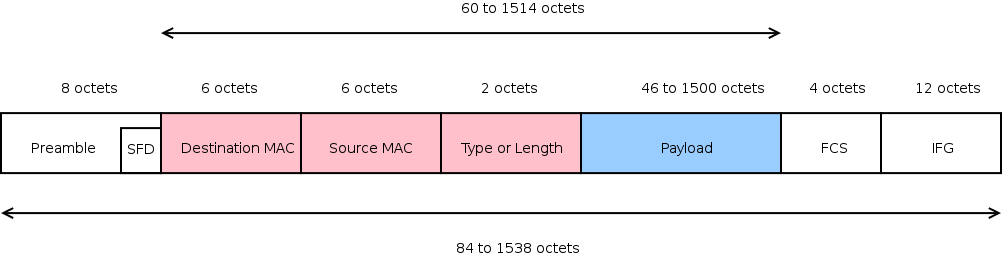
\includegraphics[width=15cm,keepaspectratio]{fig/ethernet-frame.png}
	\caption{Ethernet frame format}
	\label{fig:40gbe-ethernet-frame}
	\bigskip
\end{figure}

The Preamble, FCS and IFG carry no data and provide a necessary overhead of 24~octets for each frame.
The size of this overhead is independent from the Payload size.
Upon arrival of a frame, the rest is transferred from a network adapter to the host CPU and processed.
The data in the Ethernet header (Source and Destination MAC addresses and Type or Length) are used for L2 processing.
The data in the Payload field are used for L3 processing (i.e. routing).

The maximum sized frame is 1538 octets including the Interframe gap
(8-octet Preamble + 14-octet Ethernet header + 1500-octet Payload + 4-octet FCS + 12-octet Interframe gap).
At 40~Gbps rate, a traffic consisting of only the maximum sized frames of 1538 octets
produces $\frac{40 \times 10^{9}}{1538 \times 8} = 3~250~975$ frames per second.
In reference to the minimum frame size of 84~octets including IFG,
the 40~Gigabit Ethernet can transmit up to $\frac{40 \times 10^{9}}{84 \times 8} = 59~523~809$~frames per second.

Since each frame must be processed separately,
such high frame rates require enormous fast processing speed.
Despite the continual frame rates increases,
the 1500 byte Maximum Transmission Unit (MTU) of Ethernet remains unchanged.

Extensions to allow larger frames were made by several vendors.
The typical maximum sized jumbo frames in use are 9~038 octets (carrying 9~000 octets of Payload)~\cite{ea-jumbo-frames}.
The 40~GbE transmits $\frac{40 \times 10^{9}}{9038 \times 8} = 555~555$~of such jumbo frames per second at full rate.
